\paragraph[QuizziPedia::Front-End::Controllers\\::CreateQuestionnaireController]{QuizziPedia::Front-End::Controllers::CreateQuestionnaireController}
\begin{figure} [ht]
	\centering
	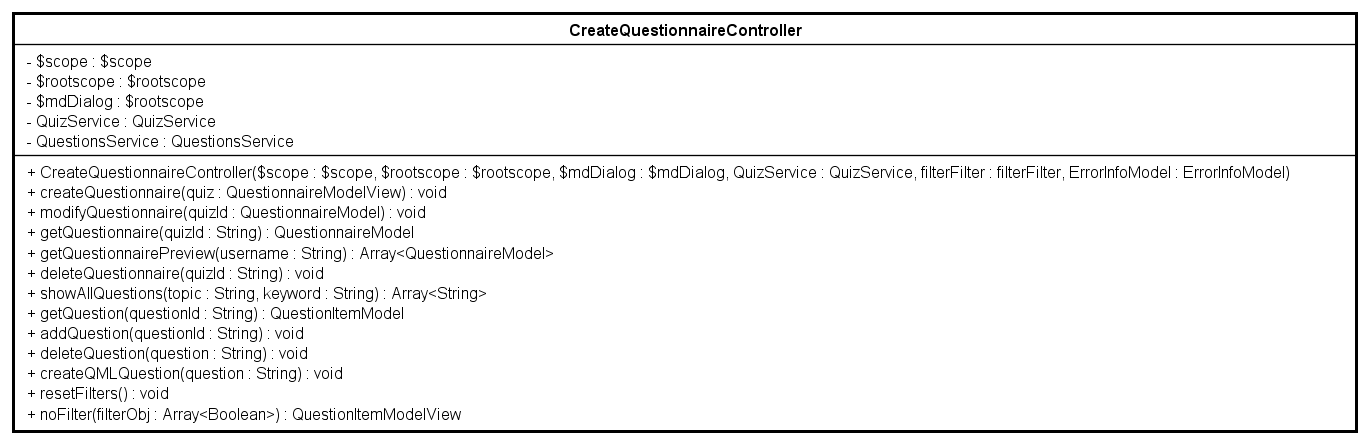
\includegraphics[scale=0.4]{UML/Classi/Front-End/QuizziPedia_Front-end_Controller_CreateQuestionnaireController.png}
	\caption{QuizziPedia::Front-End::Controllers::CreateQuestionnaireController}
\end{figure} \FloatBarrier
\begin{itemize}
	\item \textbf{Descrizione}: questa classe permette di gestire la creazione di un questionario;
	\item \textbf{Utilizzo}: fornisce tutte le funzionalità per la creazione di un nuovo questionario e per la modifica di uno esistente;
	\item \textbf{Relazione con altre classi}:
	\begin{itemize}
		\item \textbf{IN} \texttt{CreateQuestionnaireModelView}: oggetto di tipo \texttt{CreateQuestionnaireModelView}. All'interno di esso sono presenti le variabili e i metodi necessari per il \textit{Two-Way Data-Binding\ped{G}} tra la \textit{view\ped{G}} \texttt{CreateQuestionnaireView} e il \textit{controller\ped{G}} \\ \texttt{CreateQuestionnaireController}; 
		\item \textbf{IN} \texttt{QuizService}: questa classe permette di ottenere i dati di un quiz tramite delle parole chiave inserite dall'utente nella barra di ricerca;
		\item \textbf{IN} \texttt{QuestionnaireModel}: \textit{model\ped{G}} relativo ai questionari;
		\item \textbf{IN} \texttt{QuestionsService}: questa classe permette di ottenere le domande dal back-end.
	\end{itemize}
	\item \textbf{Attributi}:
	\begin{itemize}
		\item \texttt{-} \texttt{scope: Scope} \\
		Campo dati contenente un riferimento all'oggetto \$scope creato da \textit{Angular\ped{G}}, viene utilizzato come mezzo di comunicazione tra il \textit{controller\ped{G}} e la \textit{view\ped{G}}. Contiene gli oggetti che definiscono il \textit{model\ped{G}} dell'applicazione;
		\item \texttt{-} \texttt{\$rootScope: \$rootScope} \\
		Campo dati contenente il riferimento all'oggetto globale \$rootScope creato da \textit{Angular\ped{G}}. Viene utilizzato per rendere accessibile a tutti i \textit{controller\ped{G}} e a tutte le \textit{view\ped{G}} l'oggetto \texttt{QuestionnaireModel};
		\item \texttt{-} \texttt{\$mdDialog: \$mdDialog} \\
		Campo dati contenente un riferimento al servizio della libreria \textit{Material for Angular\ped{G}} che permette di creare delle componenti a pop-up;
		\item \texttt{-} \texttt{QuizService} \\ questa classe permette di ottenere i dati di un quiz tramite delle parole chiave inserite dall'utente nella barra di ricerca;
		
	\end{itemize}
	\item \textbf{Metodi}:
	\begin{itemize}
		\item \texttt{+} \texttt{CreateQuestionnaireController(\$scope: \$scope, \$rootscope: \$rootscope, \$mdDialog: \$mdDialog, QuizService: QuizService, filterFilter: filterFilter, ErrorInfoModel: ErrorInfoModel)}: \\ Metodo costruttore della classe. \\
		\textbf{Parametri}:
		\begin{itemize}
			\item \texttt{-} \texttt{\$scope: \$scope} \\
			Campo dati contenente un riferimento all'oggetto \$scope creato da \textit{Angular\ped{G}}. Viene utilizzato come mezzo di comunicazione tra il \textit{controller\ped{G}} e la \textit{view\ped{G}}. Contiene gli oggetti che definiscono il viewmodel e il \textit{model\ped{G}} dell'applicazione;
			\item \texttt{-} \texttt{\$rootScope: \$rootScope} \\
			Campo dati contenente il riferimento all'oggetto globale \$rootScope creato da \textit{Angular\ped{G}}. Viene utilizzato per rendere accessibile a tutti i \textit{controller\ped{G}} e a tutte le \textit{view\ped{G}} l'oggetto \texttt{QuestionnaireModel};
			\item \texttt{-} \texttt{\$mdDialog: \$mdDialog} \\
			Campo dati contenente un riferimento al servizio della libreria \textit{Material for Angular\ped{G}} che permette di creare delle componenti a pop-up;
			\item \texttt{-} \texttt{QuizService: QuizService}\\ Parametro che permette di ottenere, tramite il service, la lista di tutte le domande presenti nel quiz;
			\item \texttt{-} \texttt{ErrorInfoModel: ErrorInfoModel}\\ Rappresenta le informazioni di un errore che si è verificato eseguendo una determinata operazione;
			\item \texttt{-} \texttt{filterFilter: filterFilter}\\ Servizio offerto da \texttt{Angular} per effettuare dei filtri.
		\end{itemize}
		\item \texttt{+} \texttt{createQuestionnaire(quiz: QuestionnaireModelView): void}: \\Metodo che permette di inserire un questionario nel database tramite richiesta al service. \\
			\textbf{Parametri}:
			\begin{itemize}
				\item
				\texttt{quiz: QuestionnaireModel}: parametro che rappresenta l'oggetto questionario.
			\end{itemize}
		\item \texttt{+} \texttt{modifyQuestionnaire(quizId: QuestionnaireModel): void} \\ Metodo che serve per modificare un questionario. \\
			\textbf{Parametri}:
			\begin{itemize}
				\item \texttt{quiz: QuestionnaireModel}\\ Parametro che rappresenta l'oggetto questionario.
			\end{itemize}
		\item \texttt{+} \texttt{getQuestionnaire(quizId: String): QuestionnaireModel} \\Metodo che serve per ottenere un questionario tramite l'id in modo da poterlo modificare. \\
			\textbf{Parametri}:
			\begin{itemize}
				\item \texttt{quizId: String}: parametro che rappresenta l'id del questionario da richiedere.
			\end{itemize}
		\item \texttt{+} \texttt{getQuestionnairePreview(username: String): QuestionnaireModel<>} \\ Metodo che serve per ottenere la lista di tutti i questionari di un utente. \\
			\textbf{Parametri}:
			\begin{itemize}
				\item \texttt{username: String}\\ Parametro che indica l'utente del quale vogliamo caricare tutti i questionari.
			\end{itemize}
		\item \texttt{+} \texttt{deleteQuestionnaire(quizId: String): void} \\Metodo che elimina un questionario. \\
		\textbf{Parametri}:
		\begin{itemize}
			\item
			\texttt{quizId: String}\\ Identificativo del questionario da eliminare.
		\end{itemize}
		\item \texttt{+} \texttt{showAllQuestions(topic: String, keyword: String): void} \\
		Metodo che permette di ottenere la lista di tutte le domande ed inserirle nello \$scope nell'oggetto di tipo \texttt{CreateQuestionnaireModelView}.\\
		\textbf{Parametri}:
		\begin{itemize}
			\item \texttt{topic: String}\\ Parametro che indica l'argomento scelto;
			\item \texttt{keyword: String}\\ Parametro che indica la parola chiave scelta.
		\end{itemize}
		\item \texttt{+} \texttt{getQuestion(questionId: String): QuestionItemModel} \\
		Metodo che ritorna l'intera domanda selezionata.\\
		\textbf{Parametri}:
		\begin{itemize}
			\item \texttt{questionId: String}\\ Parametro che indica l'identificativo univoco di una domanda.
		\end{itemize}
		\item \texttt{+} \texttt{addQuestion(question: String) : void} \\
		Metodo che permette di inserire una domanda nel questionario.\\
		\textbf{Parametri}:
		\begin{itemize}
			\item \texttt{question: String}\\ Parametro che indica l'identificativo univoco di una domanda.
		\end{itemize}
		\item \texttt{+} \texttt{deleteQuestion(question: String) : void} \\
		Metodo che permette di rimuovere una domanda nel questionario.\\
		\textbf{Parametri}:
		\begin{itemize}
			\item \texttt{question: String}\\ Parametro che indica l'identificativo univoco di una domanda.
		\end{itemize}
		\item \texttt{+} \texttt{createQMLQuestion(question: String) : void} \\
		Metodo che permette di posizionarsi nella pagina dell'editor QML;\\
		\item \texttt{+} \texttt{filterByYours(question: String) : QuestionItemModelView} \\
		Metodo che permette di rimuovere una domanda nel questionario.\\
		\textbf{Parametri}:
		\begin{itemize}
			\item \texttt{question: String}\\ Parametro che la domanda da filtrare.
		\end{itemize}
		\item \texttt{+} \texttt{resetFilters() : void} \\
		Metodo che permette di resettare i filtri finora settati;\\
		\item \texttt{+} \texttt{noFilter(filterObj: Array<Boolean>) : QuestionItemModelView} \\
		Metodo che permette di filtrare un array.\\
		\textbf{Parametri}:
		\begin{itemize}
			\item \texttt{filterObj: Array<Boolean>}\\ Parametro contenente un array di boolean.
		\end{itemize}
	\end{itemize}
\end{itemize}

